%-----------------------------------------------------------------------------%
\chapter{\babDua}
\label{bab:2}
%-----------------------------------------------------------------------------%
Bab ini menjelaskan tinjauan kepustakaan yang digunakan dalam melakukan
penelitian ini, memuat studi akan kepustakaan serta teori-teori yang melandasi proses penelitian serta implementasi yang dilakukan.

%-----------------------------------------------------------------------------%
\section{Kontainerisasi}
\label{sec:kontainerisasiDocker}
%-----------------------------------------------------------------------------%
Menurut \cite{containerization}, kontainerisasi merupakan proses menggabungkan kode dan seluruh kebutuhan seperti library, frameworks, dan kebutuhan lainnya sehingga semuanya terisolasi kedalam sebuah 'kontainer'. Hal ini dilakukan agar aplikasi yang berjalan di dalam kontainer dapat dipindahkan dan tetap berjalan secara konsisten pada semua lingkungan dan infrastruktur, terlepas dari sistem operasi lingkungan atau infrastruktur tersebut. Kontainer bertindak sebagai "cangkang" yang membuat aplikasi dapat berjalan indipenden dari lingkungan sekitarnya.
\begin{figure}
	\centering
	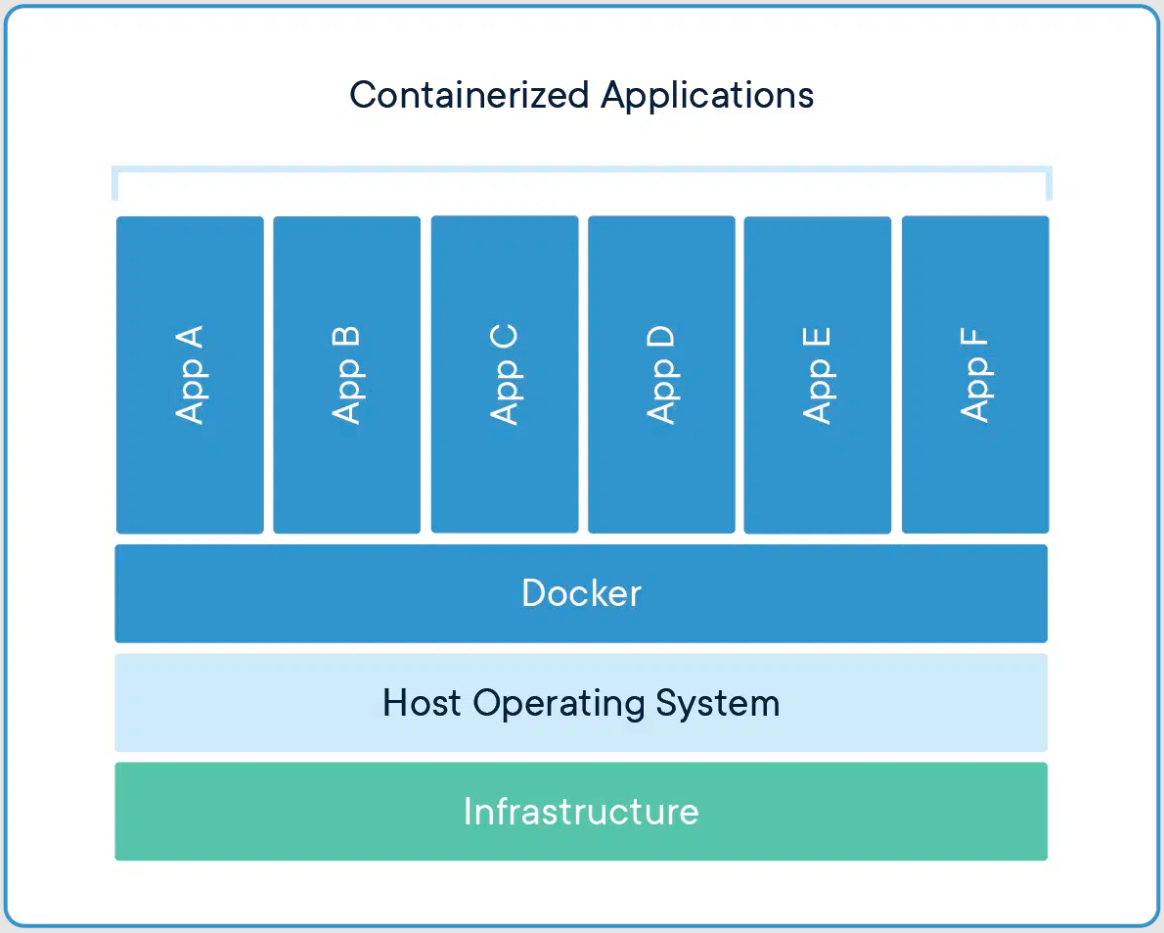
\includegraphics[width=0.8\textwidth]{pics/kontainerIlust.png}
	\caption{Ilustrasi kontainer \citep{docker_2022}}
	\label{fig:kontainer}
\end{figure}


\section{Docker}
\label{sec:dockerDef}
Docker merupakan salah satu cara untuk mengimplementasikan proses kontainerisasi. Docker diperkenalkan pada tahun 2013 dan dirilis untuk umum pada tahun 2014. Setelah kemunculannya penggunaan Docker menjadi sangat populer pada kalangan developer. Hal ini terjadi karena docker memiliki banyak keunggulan seperti: memiliki konfigurasi yang sederhana, tingkat keamanan yang baik, dan lain lain\citep{setiawan_2021}.
%-----------------------------------------------------------------------------%
\section{Kubernetes}
\label{sec:kubernetes}
%-----------------------------------------------------------------------------%
Kubernetes merupakan perangkat lunak sumber terbuka yang berguna untuk orkestrasi kontainer\citep{kubernetes}. Kubernetes dapat membantu banyak operasi seperti \textit{deployment, scaling deployment, mounting}, dan konfigurasi domain. Kontainer Docker dapat dikendalikan oleh Kubernetes.
%-----------------------------------------------------------------------------%
\section{Helm}
\label{sec:helmDef}
Helm merupakan manajer paket yang digunakan untuk mempermudah penggunaan Kubernetes\citep{merron_idowu_2020}. Dengan Helm, pengguna dapat mendefinisikan \textit{template} yang dapat dipakai untuk membuat proses modul \textit{deployment} Kubernetes menjadi lebih mudah. Definisi-definisi template beserta nilainya akan disimpan kedalam sebuah berkas yang dinamakan \code{helm chart}.
%-----------------------------------------------------------------------------%
\section{Terraform}
\label{sec:terraformDef}
Terraform adalah infrastructure as a code(IAAC) dimana pengguna dapat mendefinisikan spesifikasi \textit{deployment} pada kode\citep{terraform}. Kode tersebut kemudian akan dibaca oleh Terraform \textit{provider} yang akan melakukan \textit{deployment} sesuai dengan perintah kode. Terraform telah terintegrasi dengan banyak aplikasi seperti Kubernetes, Helm, Vault, dan fitur-fitur AWS.
%-----------------------------------------------------------------------------%
\section{Golang}
\label{sec:golang}
Go atau yang sering disebut Golang merupakan bahasa pemrograman yang dikembangkan oleh Google pada tahun 2009\citep{chris_2021}. Setelah dirilis, kepopuleran golang terus naik karena memiliki banyak keunggulan seperti: \textit{simple}, cepat, dan efisien. Golang digunakan untuk mengembangkan banyak aplikasi seperti Docker, Kubernetes, Helm, dan Vault.
%-----------------------------------------------------------------------------%
\section{Aplikasi Pihak ketiga}
\label{sec:aplikasiPihakKetiga}

Dalam dunia kerja, ada banyak aplikasi yang berjalan dan digunakan secara bersamaan. Aplikasi tersebut akan bekerja sama satu sama lain secara langsung maupun tidak langsung. Bagian ini akan membahas tentang aplikasi pihak ketiga yang akan diintegrasikan ke dalam aplikasi yaitu: Amazon S3, Amazon Kinesis, dan Vault.
%-----------------------------------------------------------------------------%
\subsection{Amazon S3}
\label{sec:amazonS3}

Amazon S3 merupakan solusi penyimpanan yang disediakan oleh Amazon\citep{chai_2021}. Amazon S3 digunakan untuk melakukan pencadangan dan penyimpanan data aplikasi pada Amazon Web Services. Amazon S3 didesain dengan sederhana untuk mempermudah proses integrasi dengan aplikasi.

%-----------------------------------------------------------------------------%
\subsection{Amazon Kinesis}
\label{sec:amazonKinesis}

Amazon Kinesis adalah message broker yang berfungsi untuk menerima data dalam bentuk \textit{stream}\citep{butts_2021}. Amazon Kinesis membantu pengguna memproses data yang masuk agar dapat diolah menjadi data yang dapat dianalisis. Setiap instance Amazon Kinesis dapat memilki banyak \textit{shards} yang masing-masingnya dapat menerima 1000 \textit{PUT request}.
%-----------------------------------------------------------------------------%
\subsection{Vault}
\label{sec:vault}

Vault merupakan sistem yang dirancang untuk dapat menyimpan rahasia secara aman dan memberikan akses kepada pihak yang berhak \citep{lugger_2020}. Rahasia yang dimaksud mencakup: \textit{password}, kunci API, kunci SSH, kunci RSA, dan lain lain. Rahasia yang tersimpan pada vault telah terenkripsi, sehingga meningkatkan keamanan dari penyimpanan tersebut.
%-----------------------------------------------------------------------------%
\section{\textit{Design Pattern}}
\label{sec:designPattern}
\textit{Design pattern} adalah solusi untuk banyak permasalahan dalam dunia pengembangan perangkat lunak\citep{shvets_2014dp}. \textit{Design pattern} bukanlah kode spesifik namun merupakan konsep umum dalam permasalahan yang spesifik. Bagian ini akan membahas beberapa \textit{design pattern} yang digunakan dalam aplikasi yang dikembangkan yaitu: \textit{Controller-Service-Repository}, dan \textit{Singleton}. 

%-----------------------------------------------------------------------------%
\subsection{\textit{Controller-Service-Repository}}
\label{sec:modelsViewController}

\textit{ControllerService-Repository} merupakan desain pattern yang didesain untuk memisahkan proses permintaan pada \textit{REST API}\citep{collings_2021}. Controller bertugas untuk membaca data dan mengubahnya menjadi data yang dapat dimengerti oleh \textit{service}. \textit{Service} berisi implementasi dari logika bisnis aplikasi. \textit{Repository} kode yang melakukan penyimpanan kedalam database.
%-----------------------------------------------------------------------------%
\subsection{\textit{Singleton}}
\label{sec:singleton}
\textit{Singleton} merupakan \textit{design pattern} yang didesain agar hanya ada satu \textit{instance} objek untuk setiap pemanggilan objek tersebut. Hal ini dilakukan agar tidak terjadinya \textit{memory leak} yang disebabkan oleh instansiasi objek yang terlalu banyak. Dengan menggunakan \textit{singleton}, pengguna hanya memiliki akses kepada \textit{getter} dari \textit{instance} tersebut yang akan mengembalikan objek jika objek tersebut sudah ada di memori, namun akan akan membuat objek baru jika objek tersebut belum ada\citep{shvets_2014st}.
%-----------------------------------------------------------------------------%
\section{Pekerjaan Terdahulu}
\label{sec:prevWork}

Terdapat pekerjaan serupa yang dikerjakan oleh \cite{microsoft_2019} yang mencoba untuk membuat API untuk melakukan \textit{deployment} Helm Chart melalui \textit{request HTTP}. Proyek ini dikembangkan mengunakan bahasa pemrograman Javascript. Sayangnya proyek ini sudah tidak lagi dikelola semenjak tahun 2019 dan kode sumbernya telah diarsipkan. 